\documentclass[border=5pt]{standalone}
\usepackage{tikz}
\usetikzlibrary{shapes,arrows.meta,positioning,backgrounds,fit,calc,matrix,decorations.pathreplacing}
\usepackage{amsmath}
\usepackage{xcolor}

% Colours
\definecolor{gridblue}{RGB}{66,133,244}
\definecolor{gridgreen}{RGB}{52,168,83}
\definecolor{gridred}{RGB}{234,67,53}
\definecolor{gridyellow}{RGB}{251,188,5}
\definecolor{gridbg}{RGB}{250,250,255}
\definecolor{arrowcol}{RGB}{100,100,120}
\definecolor{hdccol}{RGB}{171,71,188}

\begin{document}
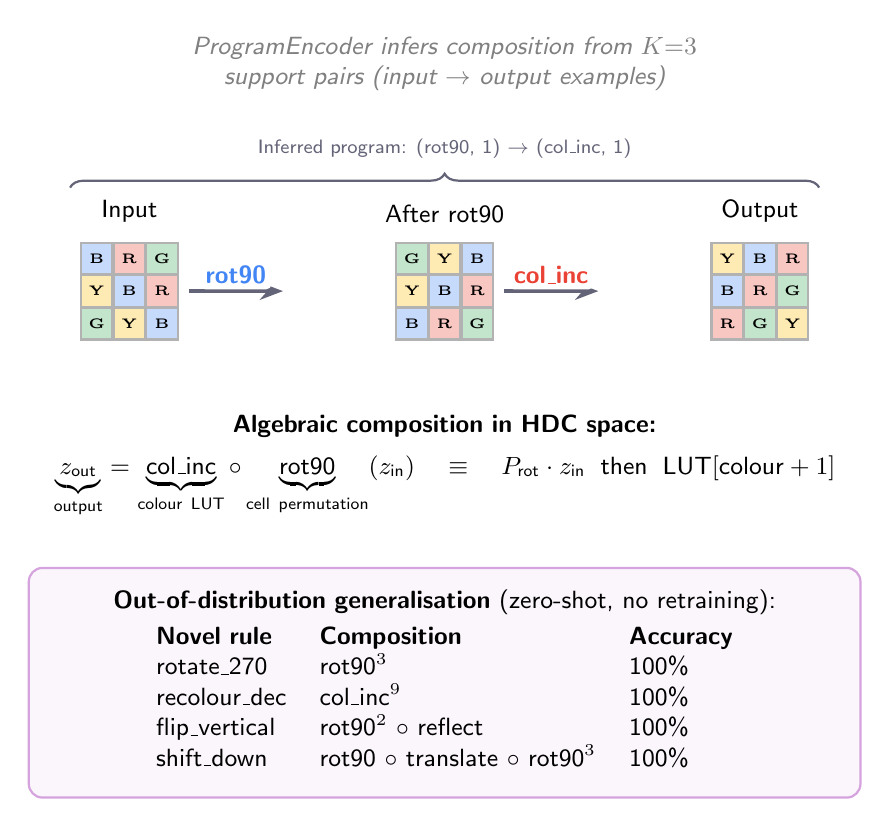
\begin{tikzpicture}[
    >=Stealth,
    gridcell/.style={minimum size=0.4cm, draw=black!30, thick, inner sep=0pt, font=\tiny\bfseries},
    arr/.style={->, very thick, color=arrowcol},
    oplabel/.style={font=\small\sffamily\bfseries, color=#1, fill=white, inner sep=2pt, rounded corners=2pt},
    steplabel/.style={font=\scriptsize\sffamily, color=black!60},
]

% ============ INPUT GRID ============
\matrix[matrix of nodes, nodes={gridcell}, column sep=-\pgflinewidth, row sep=-\pgflinewidth,
        label={[font=\small\sffamily]above:Input}] (gin) {
|[fill=gridblue!30]| B & |[fill=gridred!30]| R & |[fill=gridgreen!30]| G \\
|[fill=gridyellow!30]| Y & |[fill=gridblue!30]| B & |[fill=gridred!30]| R \\
|[fill=gridgreen!30]| G & |[fill=gridyellow!30]| Y & |[fill=gridblue!30]| B \\
};

% ============ STEP 1: ROTATION ============
\node[right=1.2cm of gin, font=\small\sffamily] (op1label) {};
\draw[arr] (gin.east) -- node[above, oplabel=gridblue] {rot90} ++(1.2,0);

\matrix[matrix of nodes, nodes={gridcell}, column sep=-\pgflinewidth, row sep=-\pgflinewidth,
        right=2.5cm of gin,
        label={[font=\small\sffamily]above:After rot90}] (g1) {
|[fill=gridgreen!30]| G & |[fill=gridyellow!30]| Y & |[fill=gridblue!30]| B \\
|[fill=gridyellow!30]| Y & |[fill=gridblue!30]| B & |[fill=gridred!30]| R \\
|[fill=gridblue!30]| B & |[fill=gridred!30]| R & |[fill=gridgreen!30]| G \\
};

% ============ STEP 2: COLOUR INCREMENT ============
\draw[arr] (g1.east) -- node[above, oplabel=gridred] {col\_inc} ++(1.2,0);

\matrix[matrix of nodes, nodes={gridcell}, column sep=-\pgflinewidth, row sep=-\pgflinewidth,
        right=2.5cm of g1,
        label={[font=\small\sffamily]above:Output}] (gout) {
|[fill=gridyellow!30]| Y & |[fill=gridblue!30]| B & |[fill=gridred!30]| R \\
|[fill=gridblue!30]| B & |[fill=gridred!30]| R & |[fill=gridgreen!30]| G \\
|[fill=gridred!30]| R & |[fill=gridgreen!30]| G & |[fill=gridyellow!30]| Y \\
};

% ============ BOTTOM: Algebraic composition ============
\node[below=0.7cm of g1, text width=10cm, align=center, font=\small\sffamily] (eq) {
\textbf{Algebraic composition in HDC space:}\\[4pt]
$\underbrace{z_{\text{out}}}_{\text{output}} = \underbrace{\text{col\_inc}}_{\text{colour LUT}} \circ \underbrace{\text{rot90}}_{\text{cell permutation}} (z_{\text{in}})
\quad\equiv\quad
P_{\text{rot}} \cdot z_{\text{in}} \;\;\text{then}\;\; \text{LUT}[\text{colour}+1]$
};

% ============ OOD GENERALISATION BOX ============
\node[below=0.5cm of eq, draw=hdccol!50, fill=hdccol!5, rounded corners=5pt, thick,
      text width=10cm, align=center, inner sep=8pt, font=\small\sffamily] (ood) {
\textbf{Out-of-distribution generalisation} (zero-shot, no retraining):\\[2pt]
\begin{tabular}{lll}
\textbf{Novel rule} & \textbf{Composition} & \textbf{Accuracy}\\
rotate\_270 & rot90$^3$ & 100\%\\
recolour\_dec & col\_inc$^9$ & 100\%\\
flip\_vertical & rot90$^2$ $\circ$ reflect & 100\%\\
shift\_down & rot90 $\circ$ translate $\circ$ rot90$^3$ & 100\%
\end{tabular}
};

% ============ BRACE: "Learned from support" ============
% raised clear of the Input/After rot90/Output matrix labels
\draw[decorate, decoration={brace, amplitude=5pt, raise=16pt}, thick, color=arrowcol]
  (gin.north west) -- (gout.north east)
  node[midway, above=23pt, font=\scriptsize\sffamily, color=arrowcol] (bracelbl) {Inferred program: (rot90, 1) $\to$ (col\_inc, 1)};

% ============ SUPPORT PAIRS ANNOTATION ============
\node[above=0.35cm of bracelbl, text width=10cm, align=center, font=\small\sffamily\itshape, color=black!50] {
  ProgramEncoder infers composition from $K{=}3$ support pairs (input $\to$ output examples)
};

\end{tikzpicture}
\end{document}
